\chapter{Testing and Evaluation}
\label{chap:eval}
\lhead{\emph{Project Testing}}
\usepackage{graphicsx}
The goal of this chapter is an objective evaluation of the final system. The evaluation must be quantitative and not qualitative. You may perform qualitative evaluation but this should not form the basis of the main conclusions you derive from the evaluation. This evaluation, where possible, should be comparative, i.e. you should evaluate your system against a commercially available system and/or system detailed in a research publication. You should demonstrate operational testing of the project using real or contrived data sets to evaluate aspects of the project not encompassed in the software testing (e.g. quantify how well does your project achieved the overall goal). 
\begin{itemize}
    \item For software based projects this will include, but should not be limited to, evaluation of non-functional requirements.
    \item For infrastructural projects this testing should include system/network KPI analysis.
    \item For analysis based projects (ML, malware or other) this may include model evaluation or YARA rule validation, for example.
    \item For management projects, where software testing or infrastructure testing may not be in scope, the test process for the system is expected to be more rigorous and well described than a project incorporating significant development work.
    \end{itemize} 
When Testing this system I conducted a select few test to ensure that this system performed the select number of tasks that was required for accurate detection of the individual.



\section{Metrics}
Identify and describe the metrics you used to evaluate your project. You should have identified some of these in the research phase report but will detail these as you progress through the design.
When Testing this system I conducted a select few test to ensure that this system performed the select number of tasks that was required for accurate detection of the individual.
1)   camera testing and haar cascade testing
2)   Testing of the haar cascade files
3)  facial recognition and identification testing through video    . 
4)   Complete system test to ensure that all components ran together and performed accurate facial detection.
It is important to note that the system is designed in a manner in which one set of functionality is added upon the previously built functionality.

\section{System Testing}

\subsection{Camera testing and video capture analysis }
The most effective method for camera testing  is to run a simple script  to activate the camera from within the pycharm working environment, along with this it is best to print put the frame which is capturing the video. A Simple script can be run to determine  if  all the opencv's packages have been installed  and imported into the working environment. 



\begin{figure}[h]
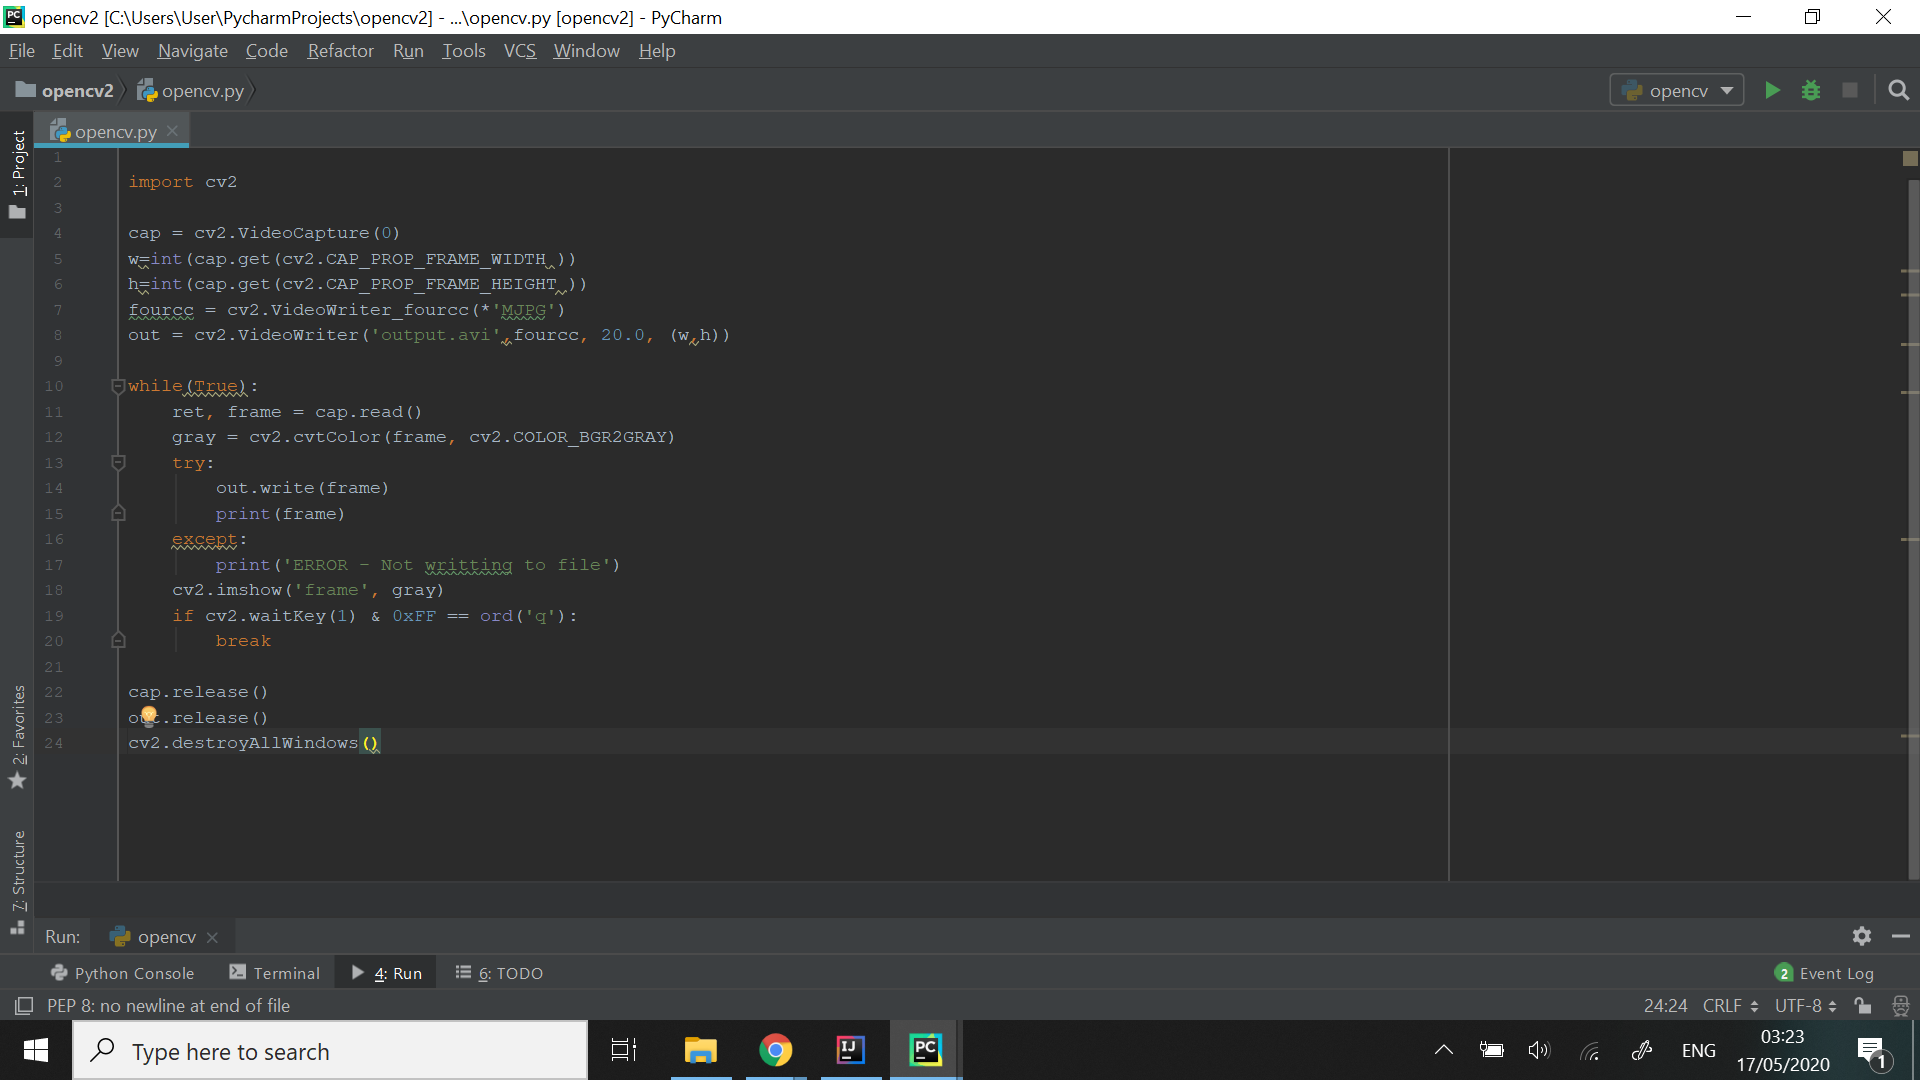
\includegraphics[width=0.5\textwidth]{Figures/videoScript.png}
\end{figure}



As you can see in the image below there is a active camera with actual video being ran of the back ground,This proves to me that opencv's packages are correctly imported into the project and is working 

\begin{figure}[h]
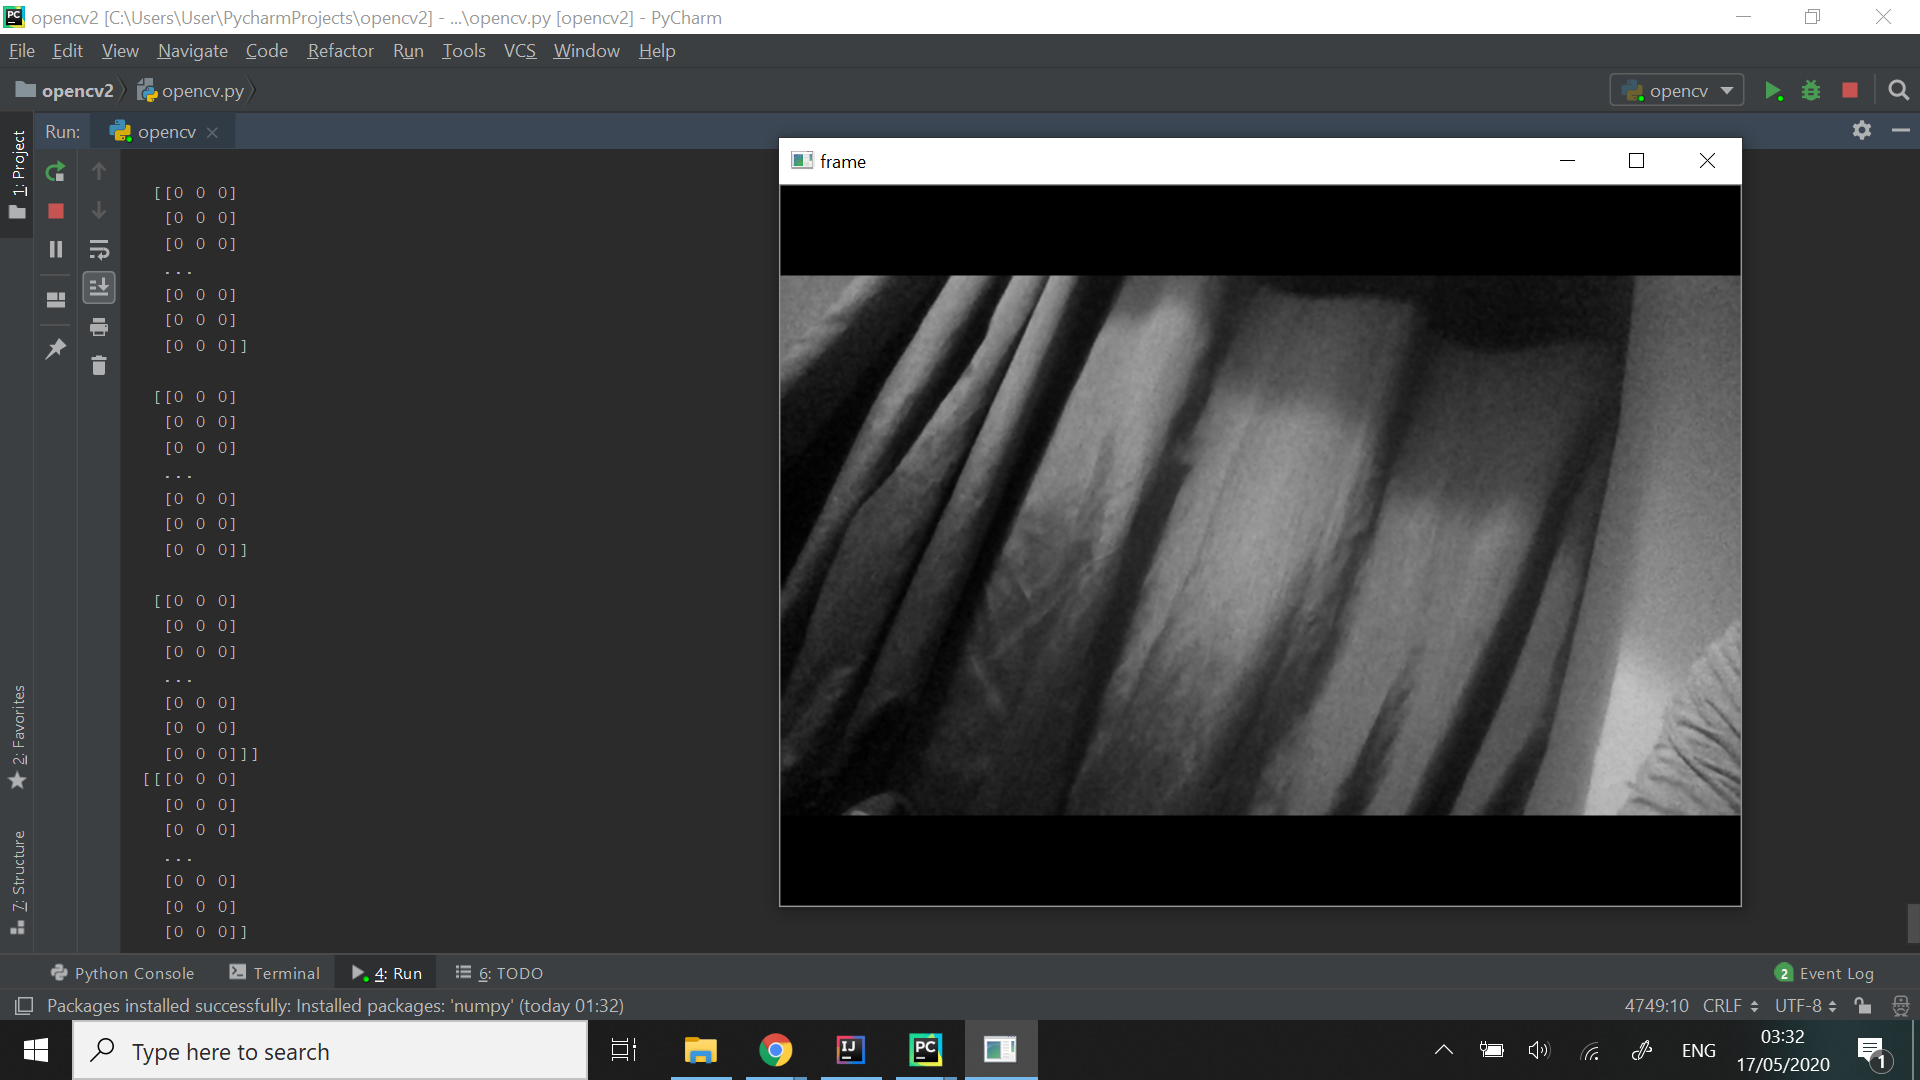
\includegraphics[width=0.7\textwidth]{Figures/video capture.png}
\end{figure}


As the opencv is configured correctly, video analysis can be done now and to perform this we need to be sure that what is being captured is being understood, the easiest way to test this is by having your script print out the values that are stored in the frame, doing this is very straight forward as you can see in the above image to the left of the video you can see that there is a matrix being printed out with the value that is being streamed into the frame. at the moment its all zeros which means nothing is being recognised by the processor. 
\begin{figure}[h]
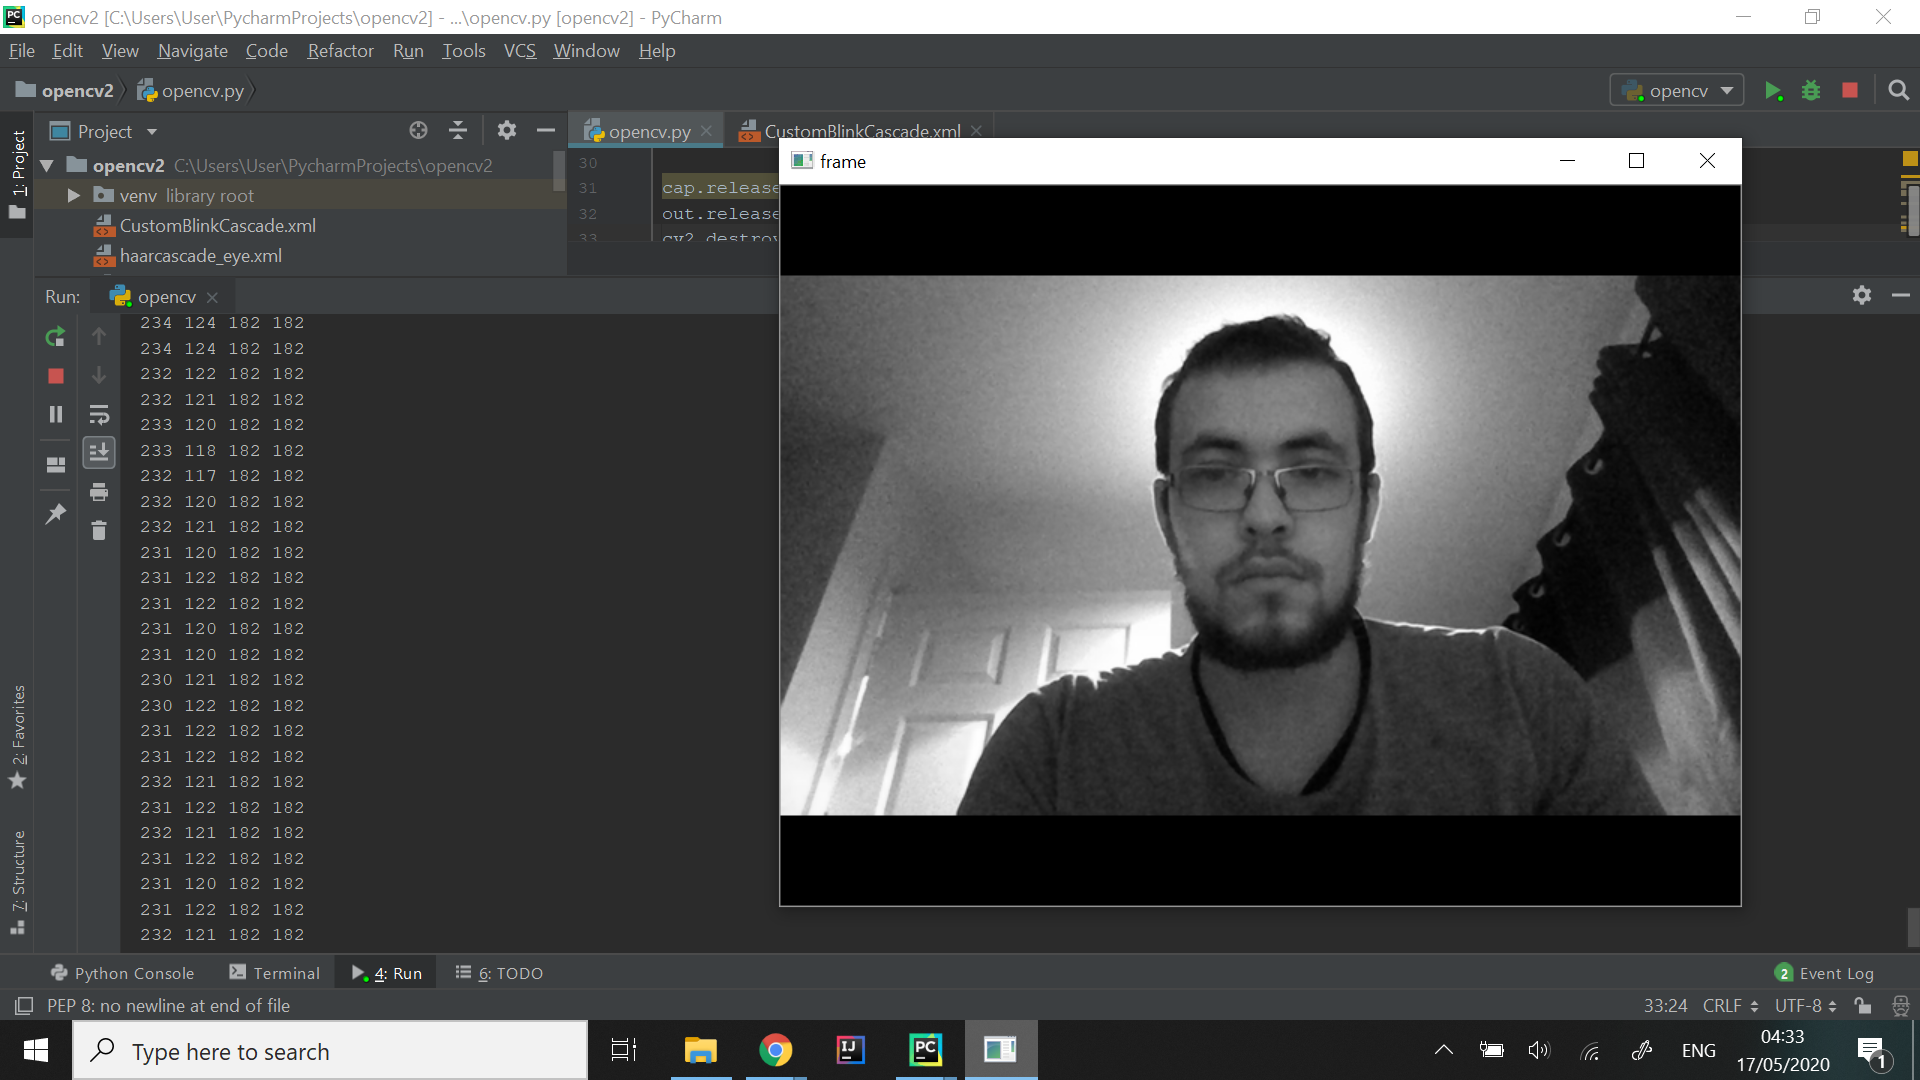
\includegraphics[width=0.8\textwidth]{Figures/videoanlysis.png}
\end{figure}
The above image show myself and beside it the matrix with validates the analysis, you can see that in previous images there was the value zero within the whole matrix and when video is analysing my face you can see that the value being printed within the matrix of myself is an infinite stream a numbers that represents me in the background of the video.
 
\subsection{Testing of the haar cascade files}
in order to test if the haar cascade files are accurately detecting my face i need to set up a test in which i must use the matrix to and python geometry to create a box around my face if the boy isn't present around my face then i can assume with great accuracy that my face isn't being detected by the haar cascade XML file. I build a script to test this.   
\begin{figure}[h]
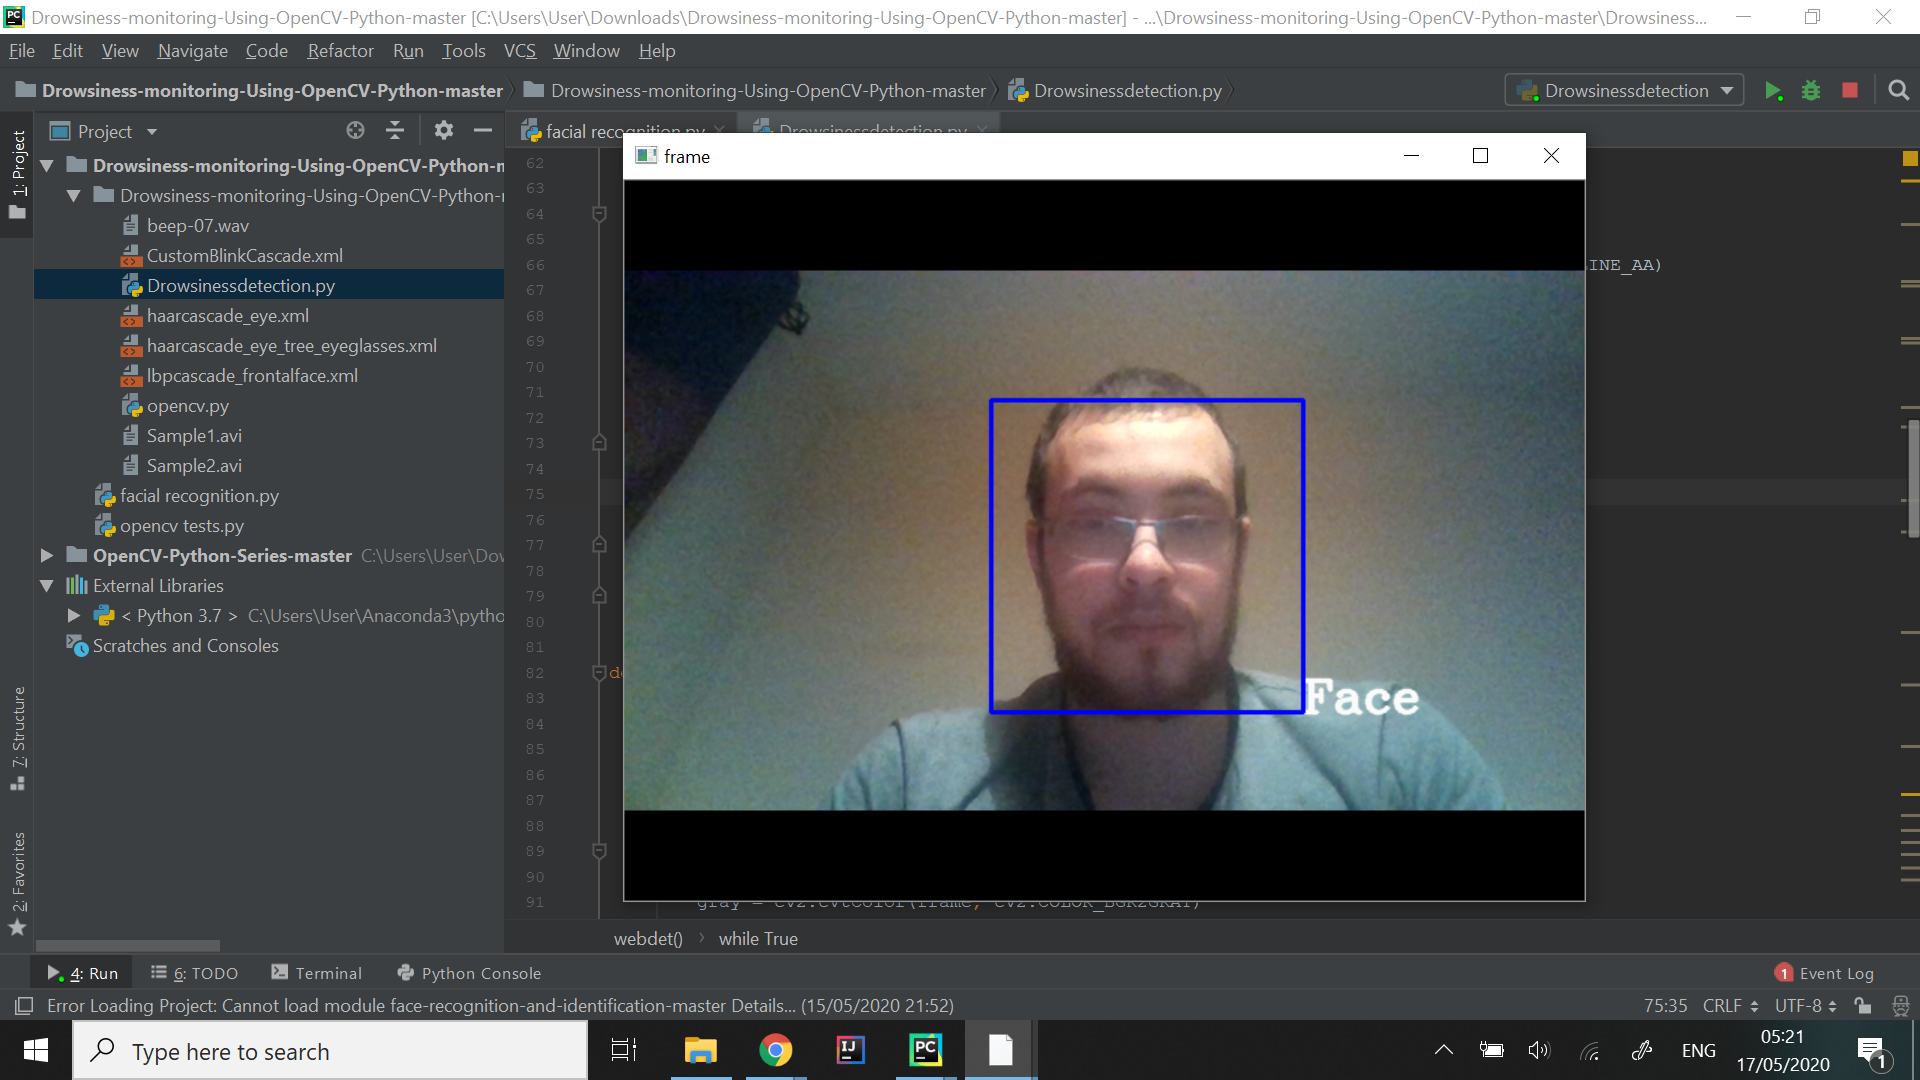
\includegraphics[width=0.8\textwidth]{Figures/facedetect.png}
\end{figure}

As you can see in the image above a blue box outlines my face which means that the haar cascade file is implemented correctly there is also a label beside it which tells me that rectangle has detected my face. The code that is highlighted is the block of that determined the face location in the video and displays a box around it. This is done by taking an x-y coordinate and setting the size of the rectangle equal to the size of the detected face that can only be detected using the cascade this then validate my test for the haar cascade being implemented properly and working 
us\begin{figure}[h]
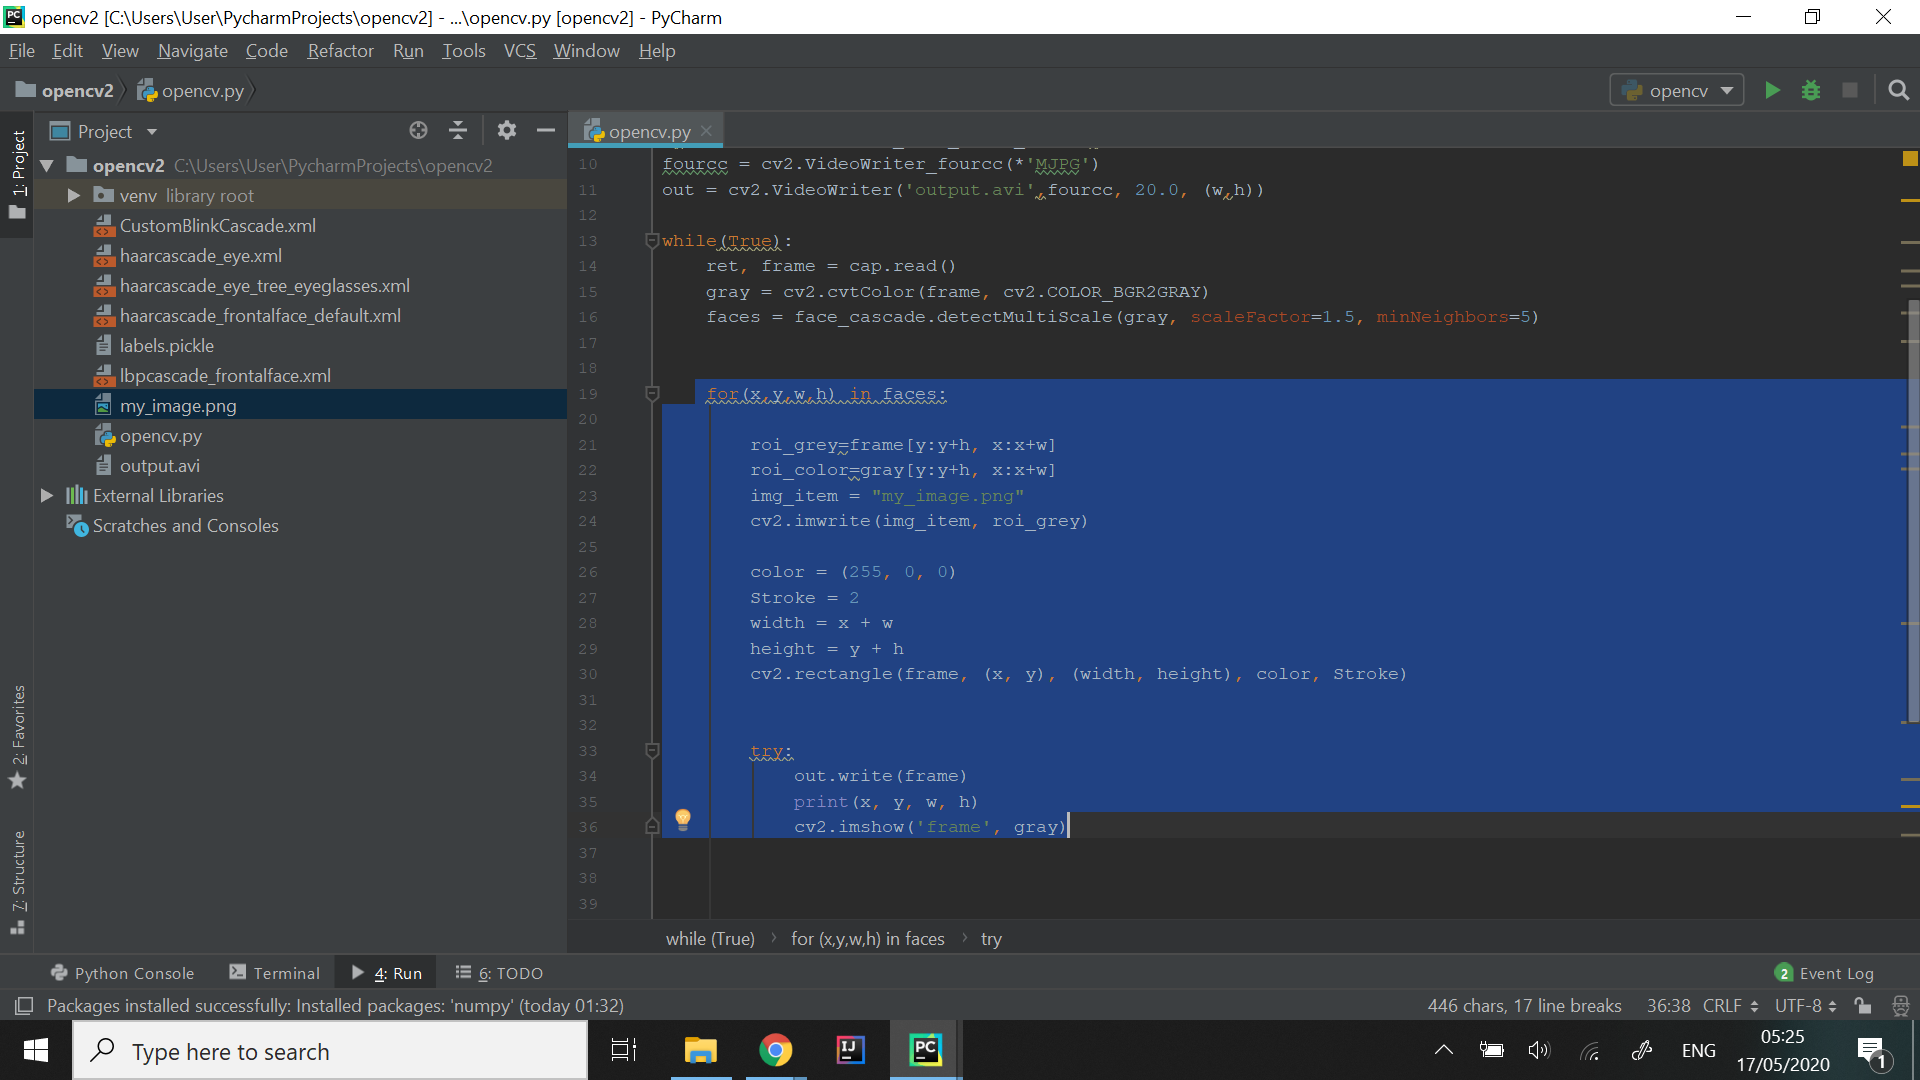
\includegraphics[width=0.8\textwidth]{Figures/facescript.png}
\end{figure}

\subsection{  Facial recognition and identification testing through video   }

when carrying out this test i made sure that i used my own image as a test for the system to identify myself and label me by my name when it has recognised me the system is performing the capture analysis of myself, I then will use other images to see if it can tell the difference between me and the random image. If my name pops up on the foreign individuals image that means the system has failed and the recognition isn't correct.

us\begin{figure}[h]
\includegraphics[width=0.8\textwidth]{Figures/facialidentification.png}
\end{figure}

As you can see by the above image the system has identified and recognised me, lets say we try another individual that as been trained by my system.


















\section{Results}
Summarise the output data, and the statistical or other techniques to deduce your results. Summarise your results, including tables or graphs as appropriate with a brief description of each. here possible, compare your results with other products/systems. Identify any possible threats to the validity of your results, and discuss each briefly here (you will discuss in more detail in the next chapter).